% 2011 年辽宁卷理科第 16 题：y=A tan(ωx+φ) 的部分图象。
% 来源 PDF：普通高考/2011/2011辽宁理.pdf，SHA-256 1fe81a3887c7782547f2dc987a468a7092be184781a1190af911ebb93a28e88e。
% 原页：第 1 页第 3 栏上部，书页码 681。图象对应 f(x)=tan(2x+π/4)。
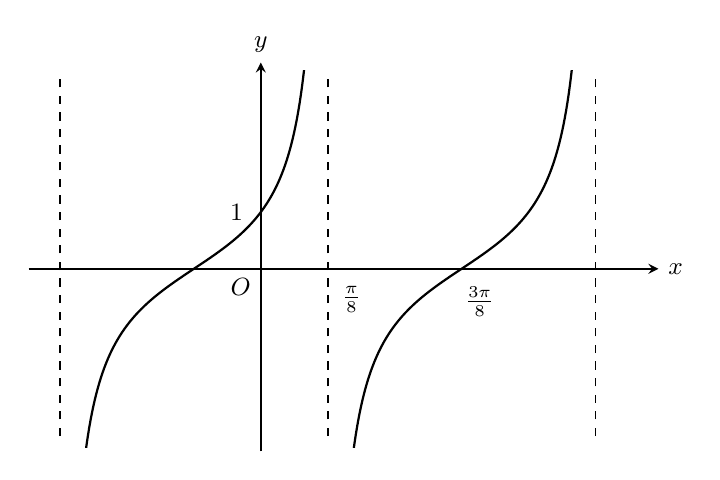
\begin{tikzpicture}[>=stealth, semithick, font=\small]
  \begin{scope}[xscale=0.85, yscale=0.72]
    \clip (-3.45,-3.15) rectangle (5.7,3.5);
    \draw[thick] plot[domain=-2.98:0.98, samples=200] (\x,{tan((\x+1)*45)});
    \draw[thick] plot[domain=1.02:4.98, samples=200] (\x,{tan((\x+1)*45)});
    \foreach \a in {-3,1,5} {
      \draw[dashed] (\a,-2.95)--(\a,3.4);
    }
  \end{scope}
  \draw[->] (-2.95,0)--(5.05,0) node[right] {$x$};
  \draw[->] (0,-2.32)--(0,2.62) node[above] {$y$};
  \node[below left] at (0,0) {$O$};
  \node[left] at (-0.1,0.72) {$1$};
  \node[below] at (1.15,-0.10) {$\frac{\pi}{8}$};
  \node[below] at (2.78,-0.10) {$\frac{3\pi}{8}$};
\end{tikzpicture}
